% Copyright 2004 by Till Tantau <tantau@users.sourceforge.net>.
%
% In principle, this file can be redistributed and/or modified under
% the terms of the GNU Public License, version 2.
%
% However, this file is supposed to be a template to be modified
% for your own needs. For this reason, if you use this file as a
% template and not specifically distribute it as part of a another
% package/program, I grant the extra permission to freely copy and
% modify this file as you see fit and even to delete this copyright
% notice. 

\documentclass{beamer}

% There are many different themes available for Beamer. A comprehensive
% list with examples is given here:
% http://deic.uab.es/~iblanes/beamer_gallery/index_by_theme.html
% You can uncomment the themes below if you would like to use a different
% one:
%\usetheme{AnnArbor}
%\usetheme{Antibes}
%\usetheme{Bergen}
%\usetheme{Berkeley}
%\usetheme{Berlin}
%\usetheme{Boadilla}
%\usetheme{boxes}
\usetheme{CambridgeUS}
%\usetheme{Copenhagen}
%\usetheme{Darmstadt}
%\usetheme{default}
%\usetheme{Frankfurt}
%\usetheme{Goettingen}
%\usetheme{Hannover}
%\usetheme{Ilmenau}
%\usetheme{JuanLesPins}
%\usetheme{Luebeck}
%\usetheme{Madrid}
%\usetheme{Malmoe}
%\usetheme{Marburg}
%\usetheme{Montpellier}
\usepackage{color}


%\usetheme{PaloAlto}
%\usetheme{Pittsburgh}
%\usetheme{Rochester}
%\usetheme{Singapore}
%\usetheme{Szeged}
%\usetheme{Warsaw}

\title{Basic Database}

% A subtitle is optional and this may be deleted
\subtitle{Midterm Project}

\author{Group.~3}
% - Give the names in the same order as the appear in the paper.
% - Use the \inst{?} command only if the authors have different
%   affiliation.

\institute[University of Science And Technology of Hanoi] % (optional, but mostly needed)
{

  \inst{}%
  University of Science And Technology of Hanoi
  \and
  \inst{}%
  ICT Department
}
% - Use the \inst command only if there are several affiliations.
% - Keep it simple, no one is interested in your street address.

\date{Thursday, April 26, 2018}

\AtBeginSubsection[]
{
  \begin{frame}<beamer>{Outline}
    \tableofcontents[currentsection,currentsubsection]
  \end{frame}
}

% Let's get started
\begin{document}

\begin{frame}
  \titlepage
\end{frame}

\begin{frame}{Outline}
  \tableofcontents
  % You might wish to add the option [pausesections]
\end{frame}

% Section and subsections will appear in the presentation overview
% and table of contents.
\section{Employee Data Query On SQL Server}

\subsection{Introduction}
\begin{frame}{Introduction}{Application}
\begin{figure}
  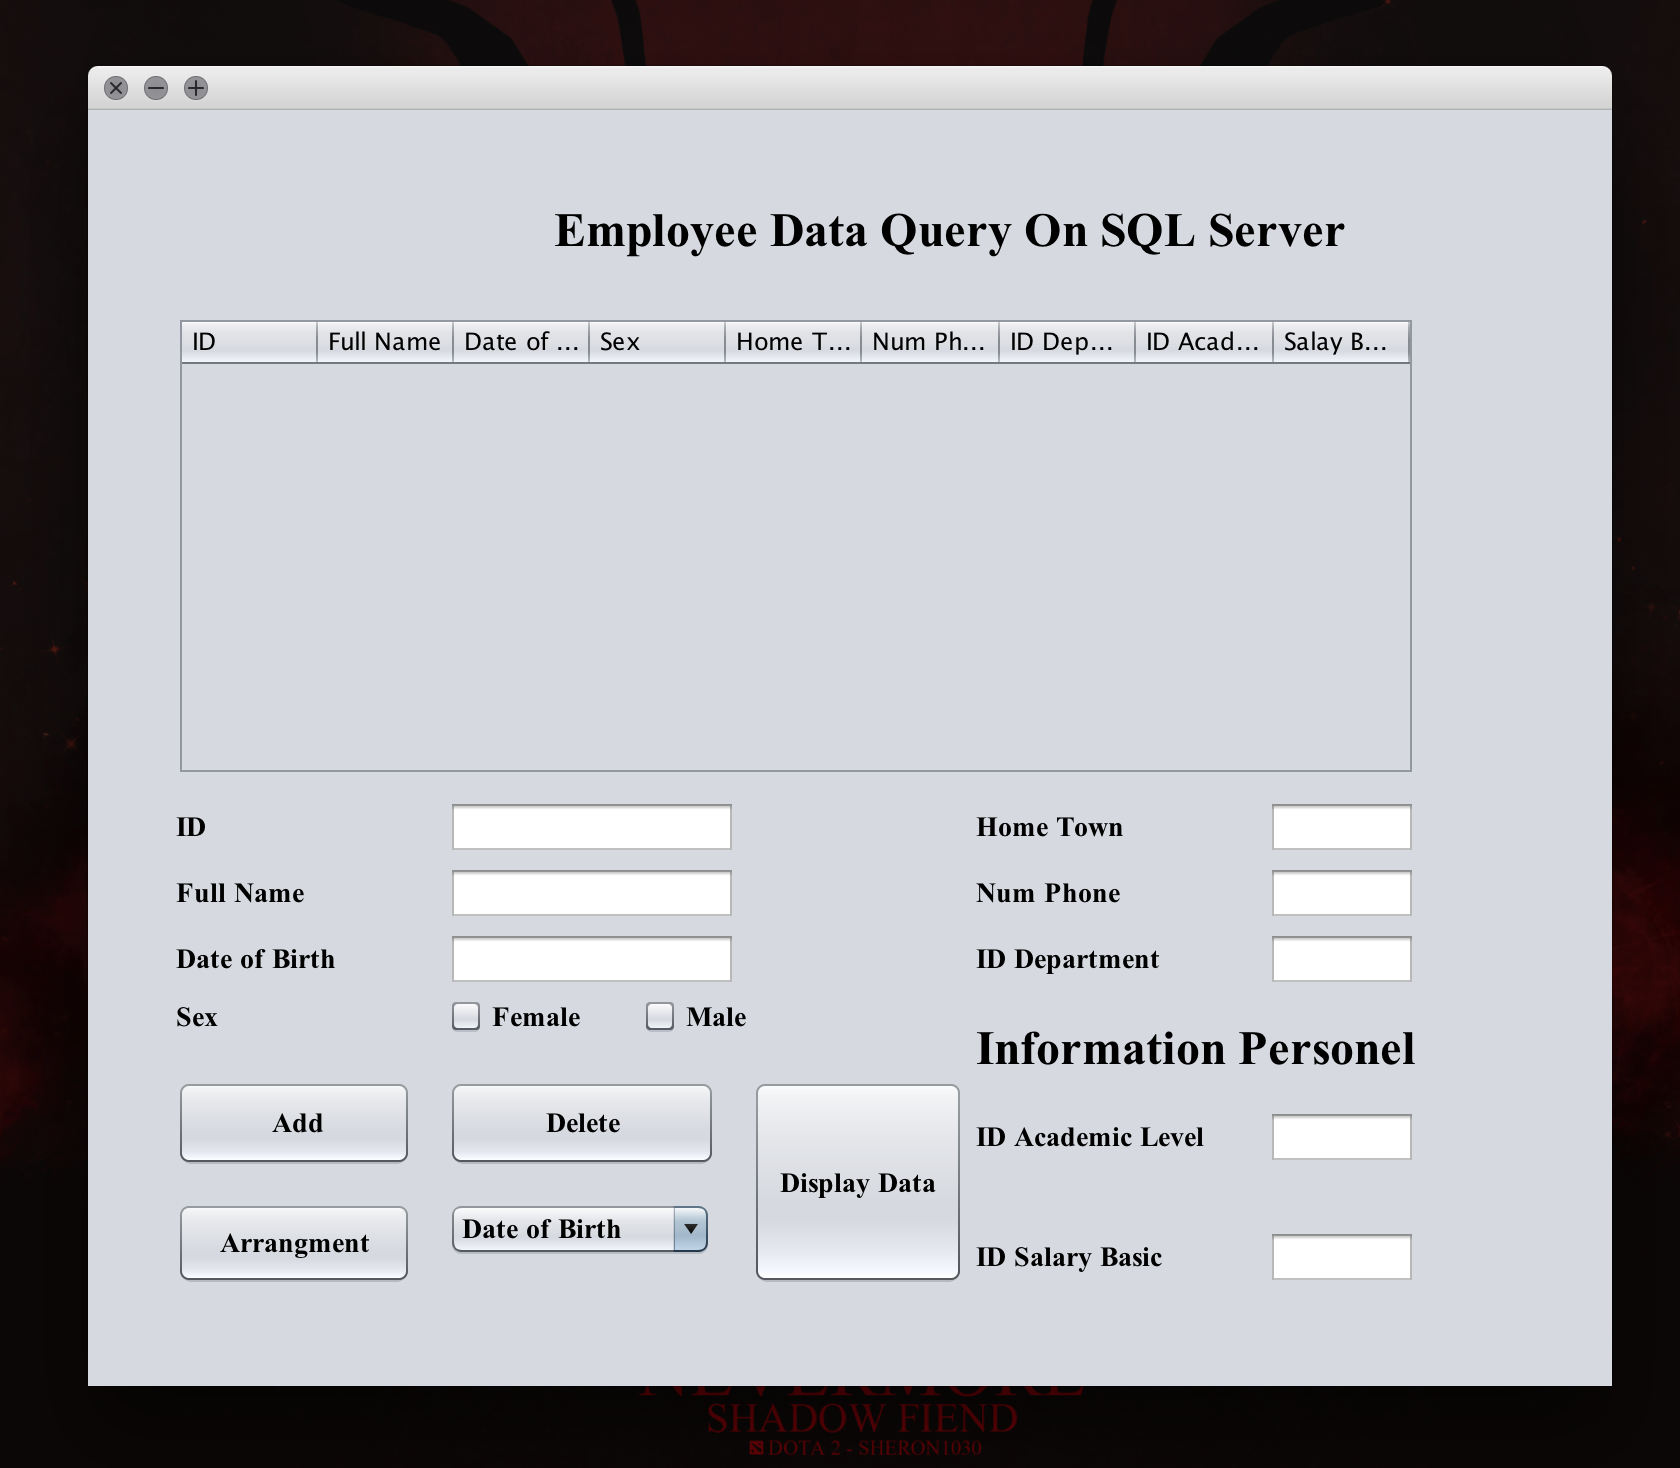
\includegraphics[scale=0.24]{1}
  \caption{Employee Data Query On SQL Server}

\end{figure}
\end{frame}

\begin{frame}{Introduction}
  \begin{itemize}
  \item {
   A Java application to manage employee.
  }
  \item {
    Swing GUI.
  }
  \item{
   SQL Sever.

  }
  \end{itemize}
\end{frame}

\subsection{Features}

% You can reveal the parts of a slide one at a time
% with the \pause command:
\begin{frame}{Features}
  \begin{itemize}
  \item {
    Java application: Write once, run anywhere
        \pause % The slide will pause after showing the first item
  }
  \item { 
    Can display all employees.  
      }
  % You can also specify when the content should appear
  % by using <n->:
  \item<3-> {
     Can add or delete.
  }
  \item<4-> {
   Sort. 
  }
  % or you can use the \uncover command to reveal general
  % content (not just \items):
  
  \end{itemize}
\end{frame}

\section{Database}

\subsection{Introduction}
\begin{frame}{Introduction}
In our application:
  \begin{itemize}
  \item {
An employee can hold multiple positions and there is may be multiple staffs work in the same positions or none.
  }
  \item {
 An employee belongs to only one department and one department may have many employees or only one employee works there.
  }
  \item{
Many employees with the same academic level and there is may have more than one employee may have same academic level.

  }
 \item{
  Many employees can be pay the same salary and there is may have more than one employee may have play with the same salary 
}
  \end{itemize}

\end{frame}

\subsection{Table}
\begin{frame}
\begin{table}
\centering
\caption{NhanVien Table.}
\begin{tabular}{llll}
Field    & Type         & Null     & Key                                                                              \\
HoTen    & nvarchar(30) & Not null &                                                                                  \\
QueQuan  & nvarchar(30) & Not null &                                                                                  \\
GioiTinh & bin          & Not null &                                                                                  \\
SDT      & char(12)     &          &                                                                                  \\
MaNV     & char(10)     & Not null & Primary Key                                                                      \\
MaLuong  & char(10)     & Not null & \begin{tabular}[c]{@{}l@{}}\\\end{tabular}                                       \\
MaTDHV   & char(10)     & Not null &                                                                                  \\
MaPB     & char(10)     & Not null & \begin{tabular}[c]{@{}l@{}}foreign key(MaPB)~\\references PhongBan\end{tabular} 
\end{tabular}
\end{table}
\end{frame}


\begin{frame}
\begin{table}
\centering
\caption{ChucVu Table}
\begin{tabular}{llll}
Field & Type         & Null     & Key                                                                                     \\
MaCV  & char(10)     & Not null & Primary Key~ ~                                                                          \\
TenCV & nvarchar(20) & Not null & \begin{tabular}[c]{@{}l@{}}foreign key(MaTDHV)~\\references TrinhDoHocVan\end{tabular} 
\end{tabular}
\end{table}
\end{frame}


\begin{frame}
\begin{table}
\centering
\caption{TrinhDoHocVan Table}
\begin{tabular}{llll}
Field       & Type                                               & Null        & Key  \\
MaTDHV      & \begin{tabular}[c]{@{}l@{}}Char(10)\\\end{tabular} & Primary Key &      \\
TenTD       & Nvarchar(20)                                       &             &      \\
ChuyenNganh & Nvarchar(20)                                       &             &     
\end{tabular}
\end{table}
\end{frame}

\begin{frame}
\begin{table}
\centering
\caption{Luong Table}
\begin{tabular}{llll}
Field      & Type     & Key      & Null         \\
MaLuong    & Char(10) & Not null & Primary Key  \\
PhuCap     & Float    &          &              \\
HSLuong    & Float    & Not null & HSLuong0     \\
LuongCoBan & Float    & Not null &             
\end{tabular}
\end{table}
\end{frame}

\begin{frame}
\begin{table}
\centering
\caption{PhongBan Table}
\begin{tabular}{llll}
Field  & Type                                                   & Key         & Null  \\
MaPB   & Char(10)                                               & Primary Key &       \\
TenPB  & Nvarchar(20)                                           &             &       \\
DiaChi & \begin{tabular}[c]{@{}l@{}}Nvarchar(30)\\\end{tabular} &             &       \\
STD    & Char(12)                                               &             &      
\end{tabular}
\end{table}
\end{frame}


\begin{frame}
\begin{table}
\centering
\caption{NhanVien\_ChucVu Table}
\begin{tabular}{llll}
Field           & Type     & Null     & Key                                                                             \\
MaNV            & char(10) & Not null & \begin{tabular}[c]{@{}l@{}}foreign key(MaNV)\\references NhanVien\end{tabular}  \\
ThoiGianCongTac & float    &          & ThoiGianCongTac > 0 \\
MaCV            & char(10) & Not null & \begin{tabular}[c]{@{}l@{}}foreign key(MaCV)\\references ChucVu\end{tabular}                                                                  
\end{tabular}
\end{table}
\end{frame}

\subsection{RDM}
\begin{frame}{RMD}
\begin{figure}
  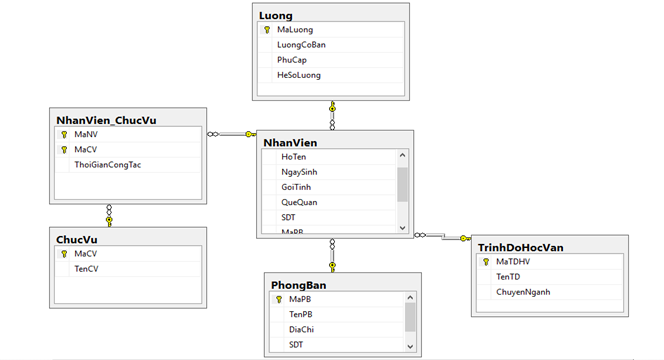
\includegraphics[scale=0.5]{2}
  \caption{RMD Figure}

\end{figure}
\end{frame}

\section*{Summary}

\begin{frame}{Summary}
  	\begin{itemize}
  		\item{
  		Check out my project on \href{https://github.com/huyhoang8398/DatabaseUSTH}{\textcolor{blue}{Github:}}\\
  			https://github.com/huyhoang8398/DatabaseUSTH
  		}
 
	\end{itemize}
\end{frame}




\end{document}


